\documentclass[
    fontsize=12pt,
    BCOR=5mm,
    DIV=12,
    parskip=half,
    listof=totoc,
    paper=a4,
    toc=bibliography,
    numbers=noenddot
]{scrreprt}

% Zentrale Konfiguration laden
% !TEX root = master.tex

%%%%%%%%%%%%%%%%%%%%%%%%%%%%%%%%%%
% PAKETE
%%%%%%%%%%%%%%%%%%%%%%%%%%%%%%%%%%

\usepackage[utf8]{inputenc}
\usepackage[T1]{fontenc}

\usepackage[ngerman]{babel}
\usepackage[german=quotes]{csquotes}

%%%%%%%%%%%%%
%% ZITIERSTIL
%%%%%%%%%%%%%
%
% @stud: Zitierstil in package biblatex unten wählen
%
% NUMERIC Style - e. g. [12]
% style=numeric 
%
% IEEE Style - numeric kind of style 
% style=ieee 
%
% ALPHABETIC Style - e. g. [AB12]
% style=alphabetic 
%
% HARVARD Style 
% style=apa 
%
% CHICAGO Style 
% style=authoryear
%
% Position des Zitats:
%
% autocite=inline 
%
% (!!) FOOTNOTE POSITION NOT RECOMMENDED IN MINT DOMAIN:
% autocite=footnote
%

\usepackage[
    backend=biber,
    autocite=inline,
    style=authoryear
]{biblatex}

% CHICAGO style (authoryear) passt

\usepackage{makeidx}
\usepackage{listings}
\usepackage{lipsum}
\usepackage{graphicx}
\usepackage[german]{varioref}
\usepackage{caption}
\usepackage{booktabs}
\usepackage[hidelinks]{hyperref}
\usepackage{fnpct}
\usepackage{calc}
\usepackage{array}
\usepackage{acronym}
\usepackage{algorithm}
\usepackage{algpseudocode}
\usepackage{setspace}
\usepackage{tocloft}
\usepackage{lmodern}
\usepackage{todonotes}
\usepackage{pdfpages}

%%%%%%%%%%%%%%%%%%%%%%%%%%%%%%%%%%
% LITERATUR
%%%%%%%%%%%%%%%%%%%%%%%%%%%%%%%%%%

\addbibresource{bibliography.bib}

\DefineBibliographyStrings{ngerman}{
    andothers = {{et\,al\adddot}},
}

%%%%%%%%%%%%%%%%%%%%%%%%%%%%%%%%%%
% SCHRIFTEN
%%%%%%%%%%%%%%%%%%%%%%%%%%%%%%%%%%

\renewcommand*{\familydefault}{\sfdefault}
\addtokomafont{disposition}{\sffamily}

%%%%%%%%%%%%%%%%%%%%%%%%%%%%%%%%%%
% FUSSNOTEN
%%%%%%%%%%%%%%%%%%%%%%%%%%%%%%%%%%

\counterwithout{footnote}{chapter}

%%%%%%%%%%%%%%%%%%%%%%%%%%%%%%%%%%
% ACRONYMS
%%%%%%%%%%%%%%%%%%%%%%%%%%%%%%%%%%

\makeatletter
\@ifpackagelater{acronym}{2015/03/20}
{\renewcommand*{\aclabelfont}[1]{\textbf{{\acsfont{#1}}}}}{}
\makeatother

%%%%%%%%%%%%%%%%%%%%%%%%%%%%%%%%%%
% LISTINGS
%%%%%%%%%%%%%%%%%%%%%%%%%%%%%%%%%%

\renewcommand{\lstlistingname}{Quelltext}
\renewcommand{\lstlistlistingname}{Quelltextverzeichnis}

\lstset{
    numbers=left,
    numberstyle=\tiny,
    captionpos=b,
    basicstyle=\ttfamily\small
}

%%%%%%%%%%%%%%%%%%%%%%%%%%%%%%%%%%
% ALGORITHMEN
%%%%%%%%%%%%%%%%%%%%%%%%%%%%%%%%%%

\renewcommand{\listalgorithmname}{Algorithmenverzeichnis}
\floatname{algorithm}{Algorithmus}

%%%%%%%%%%%%%%%%%%%%%%%%%%%%%%%%%%
% HEADER / FOOTER
%%%%%%%%%%%%%%%%%%%%%%%%%%%%%%%%%%

\RequirePackage[automark]{scrlayer-scrpage}

\renewcommand{\chaptermarkformat}{}

\RedeclareSectionCommand[
    beforeskip=0pt
]{chapter}

\clearpairofpagestyles

\ohead{\headmark}
\ofoot{\pagemark}

%%%%%%%%%%%%%%%%%%%%%%%%%%%%%%%%%%
% EIGENE BEFEHLE
%%%%%%%%%%%%%%%%%%%%%%%%%%%%%%%%%%

\newcommand{\indextype}{numeric}
\newcommand{\position}{inline}

\newcommand{\abs}{\par\vskip 0.2cm\goodbreak\noindent}
\newcommand{\nl}{\par\noindent}
\newcommand{\mcl}[1]{\mathcal{#1}}
\newcommand{\nowrite}[1]{}
\newcommand{\NN}{{\mathbb N}}
\newcommand{\imagedir}{img}

%%%%%%%%%%%%%%%%%%%%%%%%%%%%%%%%%%
% METADATEN
%%%%%%%%%%%%%%%%%%%%%%%%%%%%%%%%%%

\newcommand{\TitelDerArbeit}[1]{
    \def\DerTitelDerArbeit{#1}
    \hypersetup{pdftitle={#1}}
}

\newcommand{\AutorDerArbeit}[1]{
    \def\DerAutorDerArbeit{#1}
    \hypersetup{pdfauthor={#1}}
}

\newcommand{\Firma}[1]{\def\DerNameDerFirma{#1}}
\newcommand{\Kurs}[1]{\def\DieKursbezeichnung{#1}}
%\newcommand{\Abteilung}[1]{\def\DerNameDerAbteilung{#1}}
\newcommand{\Studiengangsleiter}[1]{\def\DerStudiengangsleiter{#1}}
\newcommand{\WissBetreuer}[1]{\def\DerWissBetreuer{#1}}
\newcommand{\FirmenBetreuer}[1]{\def\DerFirmenBetreuer{#1}}
\newcommand{\Bearbeitungszeitraum}[1]{\def\DerBearbeitungszeitraum{#1}}
\newcommand{\Abgabedatum}[1]{\def\DasAbgabedatum{#1}}
\newcommand{\Matrikelnummer}[1]{\def\DieMatrikelnummer{#1}}
\newcommand{\Studienrichtung}[1]{\def\DieStudienrichtung{#1}}
\newcommand{\ArtDerArbeit}[1]{\def\DieArtDerArbeit{#1}}
\newcommand{\Literaturverzeichnis}{Literaturverzeichnis}

%%%%%%%%%%%%%%%%%%%%%%%%%%%%%%%%%%
% HILFSFUNKTIONEN
%%%%%%%%%%%%%%%%%%%%%%%%%%%%%%%%%%

\newcommand{\setTitlepage}{
    % !TEX root =  master.tex
% @stud: ggf. Namen/Text anpassen (englisch)
\begin{titlepage}
\begin{minipage}{\textwidth}
		\vspace{-2cm}
		\noindent \includegraphics[scale=0.25]{\imagedir/firmenlogo.jpg} \hfill \includegraphics{\imagedir/logo.jpg}
\end{minipage}
\vspace{1em}
%\sffamily
\begin{center}
	{\textsf{\large Duale Hochschule Baden-W\"urttemberg Mannheim}}\\[4em]
	{\textsf{\textbf{\large{\DieArtDerArbeit}}}}\\[6mm]
	{\textsf{\textbf{\Large{}\DerTitelDerArbeit}}} \\[1.5cm]
	{\textsf{\textbf{\large{}Studiengang Wirtschaftsinformatik}}\\[6mm]
	\textsf{\textbf{Studienrichtung \DieStudienrichtung}}}\vspace{10em}
	
	\begin{minipage}{\textwidth}
		\begin{tabbing}
		Wissenschaftliche(r) Betreuer(in): \hspace{0.85cm}\=\kill
		Verfasser(in): \> \DerAutorDerArbeit \\[1.5mm]
		Matrikelnummer: \> \DieMatrikelnummer \\[1.5mm]
		Firma: \> \DerNameDerFirma  \\[1.5mm]
		%Abteilung: \> \DerNameDerAbteilung \\[1.5mm]
		Kurs: \> \DieKursbezeichnung \\[1.5mm]
		Studiengangsleiter: \> \DerStudiengangsleiter \\[1.5mm]
		Wissenschaftliche(r) Betreuer(in): \> \DerWissBetreuer \\[1.5mm]
		Firmenbetreuer(in): \> \DerFirmenBetreuer \\[1.5mm]
		Bearbeitungszeitraum: \> \DerBearbeitungszeitraum\\[1.5mm]
%		alternativ:\\[1.5mm]
%		Eingereicht: \> \DasAbgabedatum	
		\end{tabbing}
	\end{minipage}
\end{center}
\end{titlepage}
    \pagenumbering{roman}
    \normalfont
}

\newcommand{\initializeText}{
    \clearpage
    \ihead{\chaptername~\thechapter}
    \pagenumbering{arabic}
}

\newcommand{\initializeAppendix}{
    \appendix
    \ihead{}
    \cftaddtitleline{toc}{chapter}{Anhang}{}
}

\makeindex

%%%%%%%%%%%%%%%%%%%%%%%%%%%%%%%%%%%
% PERSÖNLICHE ANGABEN
%%%%%%%%%%%%%%%%%%%%%%%%%%%%%%%%%%%

\ArtDerArbeit{Projektarbeit 2}

\TitelDerArbeit{
Einsatz von LLMs zur Unterstützung von Stichprobenanalysen im Audit-Bereich. Ein Vergleich verschiedener KI-Modelle hinsichtlich ihrer Eignung für interne Prüfungsprozesse bei der Freudenberg Group
}

\AutorDerArbeit{Leonard Verclas}

%\Abteilung{xyz}

\Firma{Freudenberg \& Co. Kommanditgesellschaft}

\Kurs{WDSKI24B}

\Studienrichtung{Data Science und Künstliche Intelligenz}

\Matrikelnummer{3317974}

\Studiengangsleiter{Prof. Dr. Bernhard Drabant}

\WissBetreuer{Stefanie Bell}

\FirmenBetreuer{Andreas Hass}

\Bearbeitungszeitraum{03.08.2026 - 09.11.2026}

\Abgabedatum{09.11.2026}

%%%%%%%%%%%%%%%%%%%%%%%%%%%%%%%%%%%
% DOKUMENT
%%%%%%%%%%%%%%%%%%%%%%%%%%%%%%%%%%%

\begin{document}

\setTitlepage

%% !TEX root =  master.tex
\clearpage
\chapter*{Ehrenwörtliche Erklärung}

% Wird die folgende Zeile auskommentiert, erscheint die ehrenwörtliche
% Erklärung im Inhaltsverzeichnis.

% \addcontentsline{toc}{chapter}{Ehrenwörtliche Erklärung}
Ich versichere hiermit, dass ich die vorliegende Arbeit mit dem Titel ``\textit{\DerTitelDerArbeit}'' selbstständig verfasst und 
keine anderen als die angegebenen Quellen und Hilfsmittel benutzt habe. Ich versichere zudem, dass die eingereichte elektronische 
Fassung mit der gedruckten Fassung übereinstimmt.

\vspace{3cm}
Ort, Datum \hfill \DerAutorDerArbeit

\cleardoublepage

\chapter{Ablauf}

Frage: geht es darum, dass die LLMs bzw. der Prozess auch die Stichprobenrelevanten auswählt oder geht es um einzelne relevatne Stichproben, die alle getestet werden müssen
\begin{enumerate}
    \item Erstellen von fehlerhaften Rechnungen und Tickets (Orientierung an historischen Auditfällen)
    \item Modelle analysieren Dokumente
    \item Anwendung der Bewertungsmatrix
    \item Punktesystem auf Bewertungsmatrix anwenden
    \item Auswertung der Ergebnisse
    \item Zusätzlich: Modelle auf historische Ereignisse prüfen, bzw. historische Ereignisse nochmals auf Fehler überprüfen

\end{enumerate}


Stichprobenrisiko erklärt: (vgl. \cite[S.12]{baumeister2019sample}) und detailliert S. 40 ff.


herausforderungen und möglichkeiten künstlicher Intelligenz im Auditbereich:

Möglichkeiten:

Große datenmengen anstelle von stichproben durch schnellere Bearbeitung.
Herausfiltern von wichitgen Kennzahlen, wie kosten, vertragspartner etc.
-> Pflichtproben herausfiltern, die menschliche oder maschinelle Prüfung benötigen.
(vgl. \autocite[S.3]{KOKINA2025100734})

Anomalieerkennung -> z.b. finanzielle Informationen (vgl. \autocite[S.2]{KOKINA2025100734})

Herausforderungen:

Transparenz und Erklärbeitkeit - Auditoren und Regulatoren müssen verstehen können, warum wurde eine Entscheidung getroffen, wie ist ein Ergebnis zustande gekommen? \autocite[S.16]{KOKINA2025100734}

Robustheit und Zuverlässigkeit - Es muss nachweisbar sein, dass die Ergebnisse reproduzierbar sind, das Modlele stabil arbeiten und kein Model drift stattfindet 
\autocite[S. 13 f.]{KOKINA2025100734}

Übermäßiges Vertrauen an die KI - Auditoren müssen Ergebnisse immernoch professional skeptisch auditieren. Die Ki darf nur als Unterstützer gelten. Die finale Entscheidung bleibt beim Auditor. Durch den Einsatz von KI kann es hier zu AutomationBias führen. Hierbei kann es dazu kommen, dass Auditoren Fehler übersehen, weil das System keine gemeldet hat. \autocite[S.425 f.]{lyell2017automation}


\section{Prompt Optimiuzing}
Da die Literatur zeigt, dass die Auswahl des optimalen Prompts selbst ein schwieriges Modellselektionsproblem darstellt und die Few-Shot-Fähigkeit von LLMs häufig überschätzt wird, wurde in dieser Arbeit bewusst auf modellspezifische Promptoptimierung verzichtet. Stattdessen wurden identische Prompts für alle Modelle verwendet, um eine faire Vergleichbarkeit sicherzustellen. \cite{NEURIPS2021_5c049256}

%% !TEX root =  master.tex
\chapter*{Sperrvermerk}

\begin{center}
\fbox{
		\begin{minipage}{33em}
			\textbf{Ein Sperrvermerk sollte nur bei berechtigtem Bedarf gesetzt werden!\\[10pt] 
				Beachten Sie, dass mit Sperrvermerk	versehene Arbeiten nicht für weitere wissenschaftliche Zwecke 
				außerhalb des Firmenkontextes oder zur Publikation verwendet werden dürfen.\\[10pt]
				Wir empfehlen, wenn m\"oglich, auf den Sperrvermerk zu verzichten.\\[10pt]
				Besprechen Sie diese Problematik mit Ihrer Firma!}
		\end{minipage}
}
\end{center}

(Mustertext) Der Inhalt dieser Arbeit darf weder als Ganzes noch in Auszügen Personen außerhalb des Prüfungsprozesses 
und des Evaluationsverfahrens zugänglich gemacht werden, sofern keine anders lautende Genehmigung der Ausbildungsstätte vorliegt. 

\cleardoublepage

%\cleardoublepage

%\input{acknowledge}
\cleardoublepage

\tableofcontents
\cleardoublepage

\phantomsection
\addcontentsline{toc}{chapter}{\listfigurename}
\listoffigures
\cleardoublepage

\phantomsection
\addcontentsline{toc}{chapter}{\listtablename}
\listoftables
\cleardoublepage

\lstlistoflistings
\cleardoublepage

% !TEX root =  master.tex
\clearpage
\chapter*{Abkürzungsverzeichnis}	
\addcontentsline{toc}{chapter}{Abkürzungsverzeichnis}

\begin{acronym}[XXXXXXX]
	\acro{DHBW}{Duale Hochschule Baden-Württemberg}
	\acro{LLM}{Large Language Model}
	\acro{KI}{Künstliche Intelligenz}
	\acro{FCo}{Freudenberg \& Co.}
\end{acronym}
\cleardoublepage

\onehalfspacing

% !TEX root =  master.tex
%%
%% @stud: sprachspezifische Anpassung
%%
\chapter*{Kurzfassung (Abstract)}
\addcontentsline{toc}{chapter}{Kurzfassung (Abstract)}


\cleardoublepage

\initializeText

% !TEX root =  master.tex
\chapter{Einleitung}

\section{Problemstellung \& Motivation} 
Mit der fortschreitenden Entwicklung künstlicher Intelligenz (KI) stehen Unternehmen vor der Herausforderung, ihre Geschäftsprozesse kontinuierlich zu optimieren und durch den gezielten Einsatz neuer Technologien effizienter zu gestalten. Insbesondere im Audit-Umfeld bietet der Einsatz von KI ein erhebliches Potenzial zur Steigerung von Effizienz, Qualität und Transparenz. Die Prüfung von Dokumenten und Prozessen muss dabei zeiteffizient, nachvollziehbar und möglichst vollständig durchgeführt werden. KI kann interne Auditoren unterstützen, indem sie den manuellen Analyseaufwand reduziert und gleichzeitig umfassendere sowie schnellere Prüfungen ermöglicht (vgl. \cite[S. 11--12]{wassie2024artificial}).

Ein besonders vielversprechendes Anwendungsfeld stellt die Analyse von Audit-Stichproben dar. Im Rahmen von Prüfungen werden häufig Dokumente wie Rechnungen, User-\allowbreak Provisioning-Vorgänge oder Verträge untersucht, um Auffälligkeiten, Regelverstöße oder potenzielle Risiken zu identifizieren. Die manuelle Analyse dieser Unterlagen ist jedoch
zeitaufwendig und bindet erhebliche personelle Ressourcen. Gleichzeitig steigt aufgrund wachsender Datenmengen und zunehmend komplexer Geschäftsprozesse die Schwierigkeit,
relevante Auffälligkeiten zuverlässig zu erkennen.

Vor diesem Hintergrund gewinnt die Unterstützung von Stichprobenanalysen durch KI-basierte Verfahren zunehmend an Bedeutung. Für die Freudenberg-Gruppe als global agierendes Unternehmen stellt sich dabei die Frage, wie KI-Technologien gewinnbringend in den Internal-Audit-Prozess integriert werden können. Neben der Verbesserung der Effizienz und Prüfungsqualität spielen insbesondere die Einhaltung strenger Datenschutz- und Compliance-Anforderungen sowie die Auswahl eines geeigneten KI-Modells für die Analyse von Audit-Dokumenten eine zentrale Rolle. Daraus ergibt sich die Notwendigkeit, die Eignung verschiedener KI-Lösungen für die Unterstützung von Stichprobenanalysen im Internal Audit systematisch zu untersuchen.

\section{Zielsetzung der Arbeit}
Ziel dieser Projektarbeit ist die systematische Untersuchung der für die Stichprobenanalyse 
\section{Forschungsfrage}
Kann auch in ein Überkapitel - gibt es Unterfragen?
\section{Aufbau der Arbeit}

% !TEX root =  master.te
\chapter{Grundlagen}

\section{Audit}

Das Audit stellt eine unabhänige Prüfungsfunktion innerhalb einer Organisation dar. Die zentrale Aufgabe besteht darin die angemessene Wirksamkeit von Governance- und internen Kontrollsystemen zu bewerten und hierzu objektive Prüfungs und Beratungsleistungen bereitzustellen. (vgl. \cite[S. 263 - 264]{cantu2025making}). Dafür müssen Dokumente gesichtet, interpretiert und geprüft werden (vgl. \cite[S.556 -557]{ROUSSY2013550}). Im Rahmen dieser Arbeit liegt der Fokus auf dem Internal Audit bei \ac{FCo}, bei der Dokumente aus verschiedenen Konzernfunktionen ausgewertet werden.



\section{Stichprobenanalyse im Audit}
Für das Audit ist es in der Regel nicht möglich, alle Dokumente einer Grundgesamtheit zu prüfen. Daher wird auf die Stichprobenanalyse zurückgegriffen. Sie ist eine Prüfungsmethode im Audit-Bereich, bei der eine möglichst hohe Prüfungseffizienz erreicht werden soll. Gewählt wird demnach diejenige Handlungsalternative, die mit dem geringsten Mitteleinsatz zu einem hinreichend sicheren Prüfungsurteil führt. Aus einer Grundgesamtheit, also einer abgegrenzten Menge gleichartiger Elemente, die beispielsweise zu einem Konto gehören, werden hierzu eine Pflichtprobe und eine zufällige Stichprobe entnommen.
Die Pflichtprobe umfasst Elemente, die zuvor definierte Kriterien erfüllen, beispielsweise Rechnungen, die über einem bestimmten Betrag liegen (vgl. \cite{freudenberg2026auditsample}). Diese Elemente müssen als Teil der Stichprobe geprüft werden. Weitergehend wird aus den restlichen Elementen der Grundgesamtheit eine zufällige Stichprobe entnommen, die zusätzlich zur Pflichtprobe geprüft wird. Die verbleibenden Elemente der Grundgesamtheit werden vorerst nicht geprüft und bedingen damit eine gewisse Unschärfe der Prüfungsaussagen, die als Stichprobenrisiko bezeichnet wird (vgl. \cite[S.\,11--12]{baumeister2019sample}).

\section{Künstliche Intelligenz}

\subsection{Large Language Models}

\subsection{Prompt Engineering}

Das Prompt Engineering beschreibt den wichitgsten Part der Nutzung eines KI-Systems. Erst durch den Prompt weiß die Maschine was der User erreichen möchte. Ein Prompt kann in verschiedenen klar definierte Teile unterteilt sein.



\section{Einsatz von Künstlicher Intelligenz im Audit}

\subsection{Potenziale in der Stichprobenanalyse}

\subsection{Chancen und Risiken}

\subsection{KI-gestütze Audit-Lösungen}

DataSnipper
% !TEX root =  master.tex
\chapter{State of the Art}
\label{chap:stateoftheart}

\section{Aktuelle Durchführung von Stichprobenanalysen bei Freudenberg}
\label{sec:stichprobenanalyse_freudenberg}

Aktuell folgt die Stichprobenanalyse im Internal Audit bei Freudenberg einer strukturierten Vorgehensweise, die in den internen Vorgaben des Corporate Audit festgelegt ist (vgl. \cite{freudenberg2026auditsample}). Der Prozess lässt sich exemplarisch anhand der Prüfung von Lieferantenrechnungen ohne Bestellnummer beschreiben und ist grundsätzlich auf weitere Anwendungsfälle übertragbar. Zunächst wird eine Grundgesamtheit relevanter Objekte definiert. Im Beispiel sind das alle im Prüfungszeitraum erfassten Rechnungen ohne Bestellnummer. Anschließend wird diese Grundgesamtheit anhand definierter Kriterien, wie Rechnungswert, Lieferant, manueller Buchung oder weiterer risikorelevanter Merkmale, klassifiziert.

Auf Basis dieser Klassifizierung wird ein Schwellenwert festgelegt. Alle Rechnungen, die diesen Schwellenwert überschreiten, werden verpflichtend in die Stichprobe aufgenommen. Dieser Teil bildet die Pflichtproben ab. Ergänzend dazu wird eine zufällige Auswahl weiterer Rechnungen aus der verbleibenden Grundgesamtheit getroffen, um eine angemessene Abdeckung des Prüffeldes sicherzustellen (vgl. \cite{freudenberg2026auditsample}). Diese Kombination aus einer vollständigen Prüfung wesentlicher Elemente und einer Auswahl aus der restlichen Grundgesamtheit ist ein übliches Vorgehen bei nicht-statistischen Stichproben in der Prüfungspraxis (vgl. \cite{baumeister2019sample}).

Die ausgewählten Stichprobenelemente werden anschließend durch den Auditor einer detaillierten Prüfung unterzogen. Hierbei werden sämtliche für die Bewertung relevanten Informationen und Nachweisdokumente gesammelt, geprüft und dokumentiert. Die Global Internal Audit Standards verlangen dabei, dass die gesammelten Informationen relevant, verlässlich und ausreichend sind, um die Ergebnisse der Prüfung zu stützen (vgl. \cite[Standard~14.1]{IIA2024}). Nach Abschluss der Analyse bewertet der Auditor die Ergebnisse hinsichtlich möglicher Auffälligkeiten, Abweichungen oder Regelverstöße. Werden Unregelmäßigkeiten festgestellt, werden diese dokumentiert und als Audit Exceptions erfasst.

Durch die Kombination aus risikobasierter Auswahl und zufälliger Stichprobenziehung wird sichergestellt, dass sowohl potenziell kritische Transaktionen als auch repräsentative Elemente der Grundgesamtheit in die Prüfung einbezogen werden. Dadurch kann mit vertretbarem Prüfungsaufwand ein hohes Maß an Prüfungssicherheit erreicht werden (vgl. \cite{freudenberg2026auditsample}).


\section{Einsatz von KI im Auditbereich}

Die zuvor beschriebene Stichprobenanalyse erfolgt in weiten Teilen manuell. Für jedes Stichprobenelement sammelt, prüft und dokumentiert der Auditor die Nachweisdokumente einzeln. Genau an dieser Stelle setzt der Einsatz von \ac{KI} an. In großen Prüfungsgesellschaften sind einfache \ac{KI}-Anwendungen, etwa zur Extraktion von Informationen aus Dokumenten, bereits weit verbreitet, während komplexere Ansätze wie generative \ac{KI} bislang überwiegend experimentell eingesetzt werden (vgl. \cite[S.~2]{KOKINA2025100734}). Der Einsatz von \ac{KI} im Audit zeigt sich messbar. Prüfungsgesellschaften, die stärker in \ac{KI} investieren, erreichen eine höhere Prüfungsqualität und können gleichzeitig die Prüfungsdauer verkürzen (vgl. \cite[S.~940\,ff.]{fedyk2022}). Auch für das Internal Audit wird erwartet, dass \ac{KI} die Arbeitsweise der Prüfungsfunktion grundlegend verändert und Prüfungen effizienter macht (vgl. \cite{wassie2024artificial}). Bisher lag der Schwerpunkt vor allem auf der Analyse strukturierter Daten, beispielsweise der Erkennung von Anomalien in Finanzinformationen (vgl. \cite[S.~2]{KOKINA2025100734}). Mit generativen \acp{LLM} lassen sich nun auch unstrukturierte Dokumente wie Rechnungen, Verträge oder E-Mails auswerten. Verfahren zur Verarbeitung natürlicher Sprache werden im Internal Audit bereits für die Analyse solcher Textdaten untersucht (vgl. \cite{schumann2021natural}). Damit rückt auch die dokumentenbasierte Prüfung einzelner Stichprobenelemente in den Fokus.

Wie der Einsatz generativer \ac{KI} im Internal Audit eines Großkonzerns umgesetzt werden kann, zeigt das Beispiel Uniper. Die dortige Auditabteilung setzt ChatGPT in der Prüfungsvorbereitung, der Prüfungsdurchführung und der Berichterstattung ein. Erste Tests ergaben je nach Prozess geschätzte Effizienzgewinne von 50\,\% bis 80\,\% (vgl. \cite[S.~125\,ff.]{emett2025leveraging}). Zugleich hat Uniper eigene Regeln für die Nutzung festgelegt, da mit dem Einsatz auch Risiken verbunden sind (vgl. \cite[S.~125\,ff.]{emett2025leveraging}). Solche Risiken betreffen beim Einsatz von \ac{KI} im Audit unter anderem die Verantwortlichkeit für Ergebnisse, die Transparenz der Verfahren und den Datenschutz (vgl. \cite{munoko2020ethical}). Der Nutzen generativer \ac{KI} hängt somit von klaren Vorgaben und einer Kontrolle der Nutzung und der Ergebnisse ab.

\section{Verfügbare KI-Lösungen für den Auditbereich}
\label{sec:ki_loesungen}

Für den Einsatz von \ac{KI} im Auditbereich stehen verschiedene Arten von Lösungen zur Verfügung. Diese lassen sich in drei Gruppen einteilen: kommerzielle \acp{LLM}, die von Anbietern wie Anthropic, OpenAI oder Google bereitgestellt werden, Open-Source-Modelle, die auf eigener Infrastruktur betrieben werden können, sowie spezialisierte Softwarelösungen, die gezielt für Prüfungsprozesse entwickelt wurden. Im Folgenden werden diese drei Gruppen vorgestellt und hinsichtlich Leistungsfähigkeit, Datenschutz, Kosten und Implementierungsaufwand eingeordnet.

\subsection{Kommerzielle Lösungen}
\label{subsec:kommerziell}

Generative \ac{KI} und speziell \acp{LLM} werden in der Forschung zunehmend als neue Allzwecktechnologie eingeordnet, die in vielen Branchen und Tätigkeiten eingesetzt werden kann (vgl. \cite{calvino2025generative}). Damit kommen \acp{LLM} grundsätzlich auch für den Einsatz im Auditbereich in Frage. Generative \acp{LLM} sind in der Lage, große Mengen an Textdaten zu verarbeiten, Muster zu erkennen und Informationen aus unstrukturierten Dokumenten wie Rechnungen strukturiert wiederzugeben, was für die Prüfung von Stichproben im Auditbereich relevant ist. Jedoch ist zu berücksichtigen, dass die Modelle auch halluzinieren können, also falsche oder nicht belegbare Informationen generieren (vgl. \cites[S.~2]{ji2023hallucination}[S.~2]{huang2025survey}[S.~1]{bang2025hallulens}). Daher ist eine abschließende Bewertung der Ergebnisse durch den Auditor weiterhin erforderlich.

Die einzelnen Modelle werden kontinuierlich weiterentwickelt, wobei ihre Leistungsfähigkeit und Genauigkeit stetig zunimmt (vgl. \cite{ArtificialAnalysis2026}). Zum Stand der Arbeit (Ok~tober~2026) führen Modelle von Anthropic, OpenAI und Google die Benchmark-Rankings wie den Artificial Analysis Intelligence Index an. Modelle wie Claude Opus 5.5, Claude Sonnet 5.5, Claude Fable 5.1, GPT-6 Astra und Gemini 4 schneiden hierbei am besten ab (vgl. \cite{ArtificialAnalysis2026}). Der Artificial Analysis Intelligence Index kann jedoch nur als erster Referenzwert herangezogen werden (vgl. \cite{thebatch2026aaindex}). Für den konkreten Anwendungsfall der Stichprobenanalyse im Audit sind weitere, spezifische Faktoren zu berücksichtigen, die im Rahmen der Evaluation untersucht werden.

Kommerzielle Modelle werden in der Regel als Cloud-Dienst bereitgestellt. Sie lassen sich mit geringem Implementierungsaufwand nutzen, die Verarbeitung der Daten erfolgt jedoch auf der Infrastruktur des Anbieters. Für den Einsatz mit vertraulichen Prüfungsdaten ist daher ein vertraglich abgesicherter Zugang notwendig, wie er bei Freudenberg über den Microsoft Copilot besteht (vgl. \cite{Microsoft2026CopilotPrivacy}).

\subsection{Open-Source-Lösungen}
\label{subsec:opensource}

Neben kommerziellen Modellen existieren Open-Source-Modelle. Als Open-Source-Modelle werden \acp{LLM} verstanden, deren Modellgewichte frei verfügbar sind (vgl. \cite[S.~2]{kapoor2024openfm}). Bekannte Beispiele sind Llama von Meta, die Modelle von Mistral, Qwen von Alibaba, Kimi von Moonshot AI oder DeepSeek (vgl. \cite{ArtificialAnalysis2026}).
Open-Source-Modelle stellen grundsätzlich eine Alternative zu kommerziellen Lösungen dar. Durch den Betrieb auf unternehmensinterner Infrastruktur verlassen die Daten das Unternehmen nicht, wodurch Datenschutz- und Compliance-Anforderungen gezielt berücksichtigt werden können (vgl. \cite[S.~3]{kapoor2024openfm}). Zudem fallen keine nutzungsabhängigen Lizenzkosten an (vgl. \cite[S.~9]{kapoor2024openfm}).

Dem steht ein erheblicher Infrastruktur- und Implementierungsaufwand gegenüber. Für den Betrieb leistungsfähiger Modelle wird eigene Hardware mit ausreichender Rechenleistung benötigt. Hinzu kommen die Wartung, die Aktualisierung der Modelle und das notwendige Fachwissen im Unternehmen (vgl. \cite[S.~3]{kapoor2024openfm}). Außerdem liegen in den aktuellen Benchmark-Rankings die kommerziellen Modelle vor Open-Source Lösungen (vgl. \cite{ArtificialAnalysis2026}).

\subsection{Spezialisierte KI-gestützte Audit-Lösungen}
\label{subsec:spezialisiert}

Abseits von generativen \acp{LLM} existieren spezialisierte Softwarelösungen, die \ac{KI} gezielt für Prüfungsprozesse einsetzen. Ein bekanntes Beispiel dafür ist DataSnipper. Die Software erzielt auf Bewertungsplattformen gute Bewertungen (vgl. \cites{GartnerPeerInsights_DataSnipper_2026}) und wird laut Hersteller unter anderem von den Big 4 eingesetzt, wodurch sie eine hohe Marktrelevanz im Prüfungsumfeld besitzt (vgl. \cite{DataSnipper_AboutUs_2026}). DataSnipper ist als Erweiterung für Microsoft Excel umgesetzt und wurde speziell für die Anforderungen von Prüfungs- und Finanzprozessen entwickelt (vgl. \cite{YourAIFinder_DataSnipper_2026}). Zu den zentralen Funktionen gehören die automatisierte Extraktion von Daten aus Dokumenten, der Abgleich dieser Daten mit Arbeitspapieren sowie die Erstellung nachvollziehbarer Audit Trails. Fachliche Entscheidungen und die finale Bewertung verbleiben dabei weiterhin beim Auditor (vgl. \cite{G2_DataSnipper_2026}).

Spezialisierte Lösungen sind auf typische Prüfungsschritte zugeschnitten und lassen sich ohne eigene Prompt-Entwicklung nutzen. Sie sind jedoch an den Funktionsumfang des Herstellers gebunden und erfordern in der Regel eine zusätzliche Lizenz.

\section{Einordnung des KI-Einsatzes bei Freudenberg}
\label{sec:ki_at_the_moment}

Die Freudenberg Gruppe nutzt aktuell gruppenweit die \ac{KI}-Lösung von Microsoft, den Microsoft Copilot. Hierbei werden für alle Nutzer die Modelle GPT-5.6, GPT-6.1 sowie Claude Sonnet 5, Claude Sonnet 5.5 und Claude Opus 5.5 zur Verfügung gestellt (vgl. \cite{freudenberg2026copilot}). Der Copilot kann dabei unter Berücksichtigung der Datenschutz- und Compliance Richtlinien auf alle internen Dokumente zugreifen, für die der jeweilige Nutzer berechtigt ist. Zusätzlich bietet Microsoft die Möglichkeit, über das Copilot Studio eigene Agenten zu bauen. Hierbei können die Agenten auf interne Dokumente zugreifen und Aufgaben automatisiert ausführen. Für die Agenten sind aktuell die Modelle GPT-4.1, GPT-5, GPT-5.3, GPT-5.5 sowie Claude Sonnet 4.6, Claude Opus 4.6, Claude Opus 4.7 und Claude Opus 4.8 hinterlegt (vgl. \cite{freudenberg2026copilot}).

Für die Stichprobenanalyse von Rechnungen im Auditkontext empfiehlt sich der Einsatz eigener Agenten im Copilot Studio anstelle der reinen Chatnutzung des Microsoft Copilot. Der Grund liegt im Aufbau des Prüfprozesses. Wie in Abschnitt \ref{sec:stichprobenanalyse_freudenberg} beschrieben, besteht die Stichprobenanalyse aus mehreren aufeinander aufbauenden Schritten, die für jedes Stichprobenelement wiederholt werden. Es müssen Nachweisdokumente gesammelt werden, mit den Buchungsdaten abgeglichen werden, Auffälligkeiten identifiziert werden und das Ergebnis dokumentiert werden.

Grundsätzlich lassen sich alle Prüfschritte auch in einem einzelnen, ausführlichen Prompt im Microsoft Copilot beschreiben. Sprachmodelle reagieren jedoch empfindlich auf kleine Unterschiede in der Formulierung und Formatierung eines Prompts (vgl. \cite[S.~16]{ICLR2024_6c0e99d7}). Dienen unterschiedliche Dokumente als Grundlage, können dadurch voneinander abweichende Ergebnisse entstehen. Bei einer größeren Anzahl an Stichprobenelementen kommt hinzu, dass ein einzelner Chatverlauf schnell sehr lang wird. Informationen in der Mitte langer Kontexte werden von den Modellen schlechter berücksichtigt (vgl. \cite[S.~157]{liu2024lost}) und irrelevante Inhalte können die Ergebnisse zusätzlich verschlechtern (vgl. \cite{shi2023distracted}). Frühere Anweisungen können dadurch an Wirkung verlieren. Für eine Prüfung, deren Ergebnisse nachvollziehbar und vergleichbar sein müssen, ist das ein Nachteil.

Ein Agent wird dagegen einmalig mit festen Anweisungen, definierten Wissensquellen und den benötigten Aktionen konfiguriert (vgl. \cite{microsoft2026declarative}). Dadurch läuft jede Rechnung nach demselben Schema durch die Prüfung, und der Ablauf lässt sich dokumentieren und wiederverwenden. \textcite[S. 1]{schreyer2024agentic} beschreiben diesen Schritt als Übergang vom co-piloted Auditing, bei dem ein \ac{LLM} einzelne Aufgaben auf Anfrage unterstützt, zum auto-piloted Auditing, bei dem Agenten zusammenhängende Prüfungshandlungen eigenständig ausführen. \todo{eine quelle ist hier für den ansatz sehr entscheidend. Ist die Quelle so stark?}

Gleichzeitig besteht im Copilot Studio aktuell die Einschränkung, dass dort ältere Modelle zur Verfügung stehen als im Chatfenster des Microsoft Copilot. Für den vorliegenden Anwendungsfall ist jedoch weniger die maximal mögliche Modellleistung entscheidend als vielmehr ein standardisierter und reproduzierbarer Prüfungsablauf. Die Verwendung eines Agenten ermöglicht eine konsistente Verarbeitung aller Stichprobenelemente sowie eine bessere Nachvollziehbarkeit der Ergebnisse. \todo{Quelle} 

Unabhängig vom gewählten Modell verbleibt die fachliche Verantwortung für die Beurteilung der Ergebnisse weiterhin beim Auditor. Dabei besteht jedoch das Risiko des Automation Bias. Nutzer vertrauen den Ergebnissen automatisierter Systeme zu stark und können dadurch Fehler leichter übersehen (vgl. \cite[S.~425 f.]{lyell2017automation}). Die vom Agenten erzeugten Ergebnisse sind daher als Entscheidungshilfe zu verstehen und müssen durch den Auditor eigenständig überprüft werden.

Zusammenfassend bietet der Einsatz eines Agenten im Microsoft Copilot Studio für die Stichprobenanalyse von Rechnungen im Auditkontext Vorteile hinsichtlich Standardisierung, Wiederverwendbarkeit und Nachvollziehbarkeit des Prüfprozesses. Der Agent kann auf die für die Prüfung relevanten Dokumente zugreifen, Informationen extrahieren und die definierten Prüfschritte automatisiert durchführen. Offen bleibt jedoch, welches der verfügbaren Modelle für diesen Anwendungsfall die besten Ergebnisse liefert. Zur Beantwortung dieser Frage wird im weiteren Verlauf der Arbeit eine Evaluation durchgeführt, in der die Leistungsfähigkeit der verfügbaren Modelle verglichen wird.

% !TEX root =  master.tex
\chapter{Fazit und Ausblick}

\section{Zusammenfassung der wichtigsten Erkenntnisse}

\section{Fazit zur Eignung von LLMs im Audit}

\section{Handlungsempfehlungen für Freudenberg}

\section{Zukünfige Entwicklungspotenziale}

\initializeAppendix

% !TEX root =  master.tex
\chapter{Prompts}

\section{Prompt GPT}

\lipsum


\section{Prompt Claude}

\lipsum

% !TEX root =  master.tex
\chapter{Beispiel-Anhang: Noch ein Testanhang}
nochmal: lipsum ...


\singlespacing

\printbibliography

\cleardoublepage

%\addcontentsline{toc}{chapter}{Index}
%\printindex

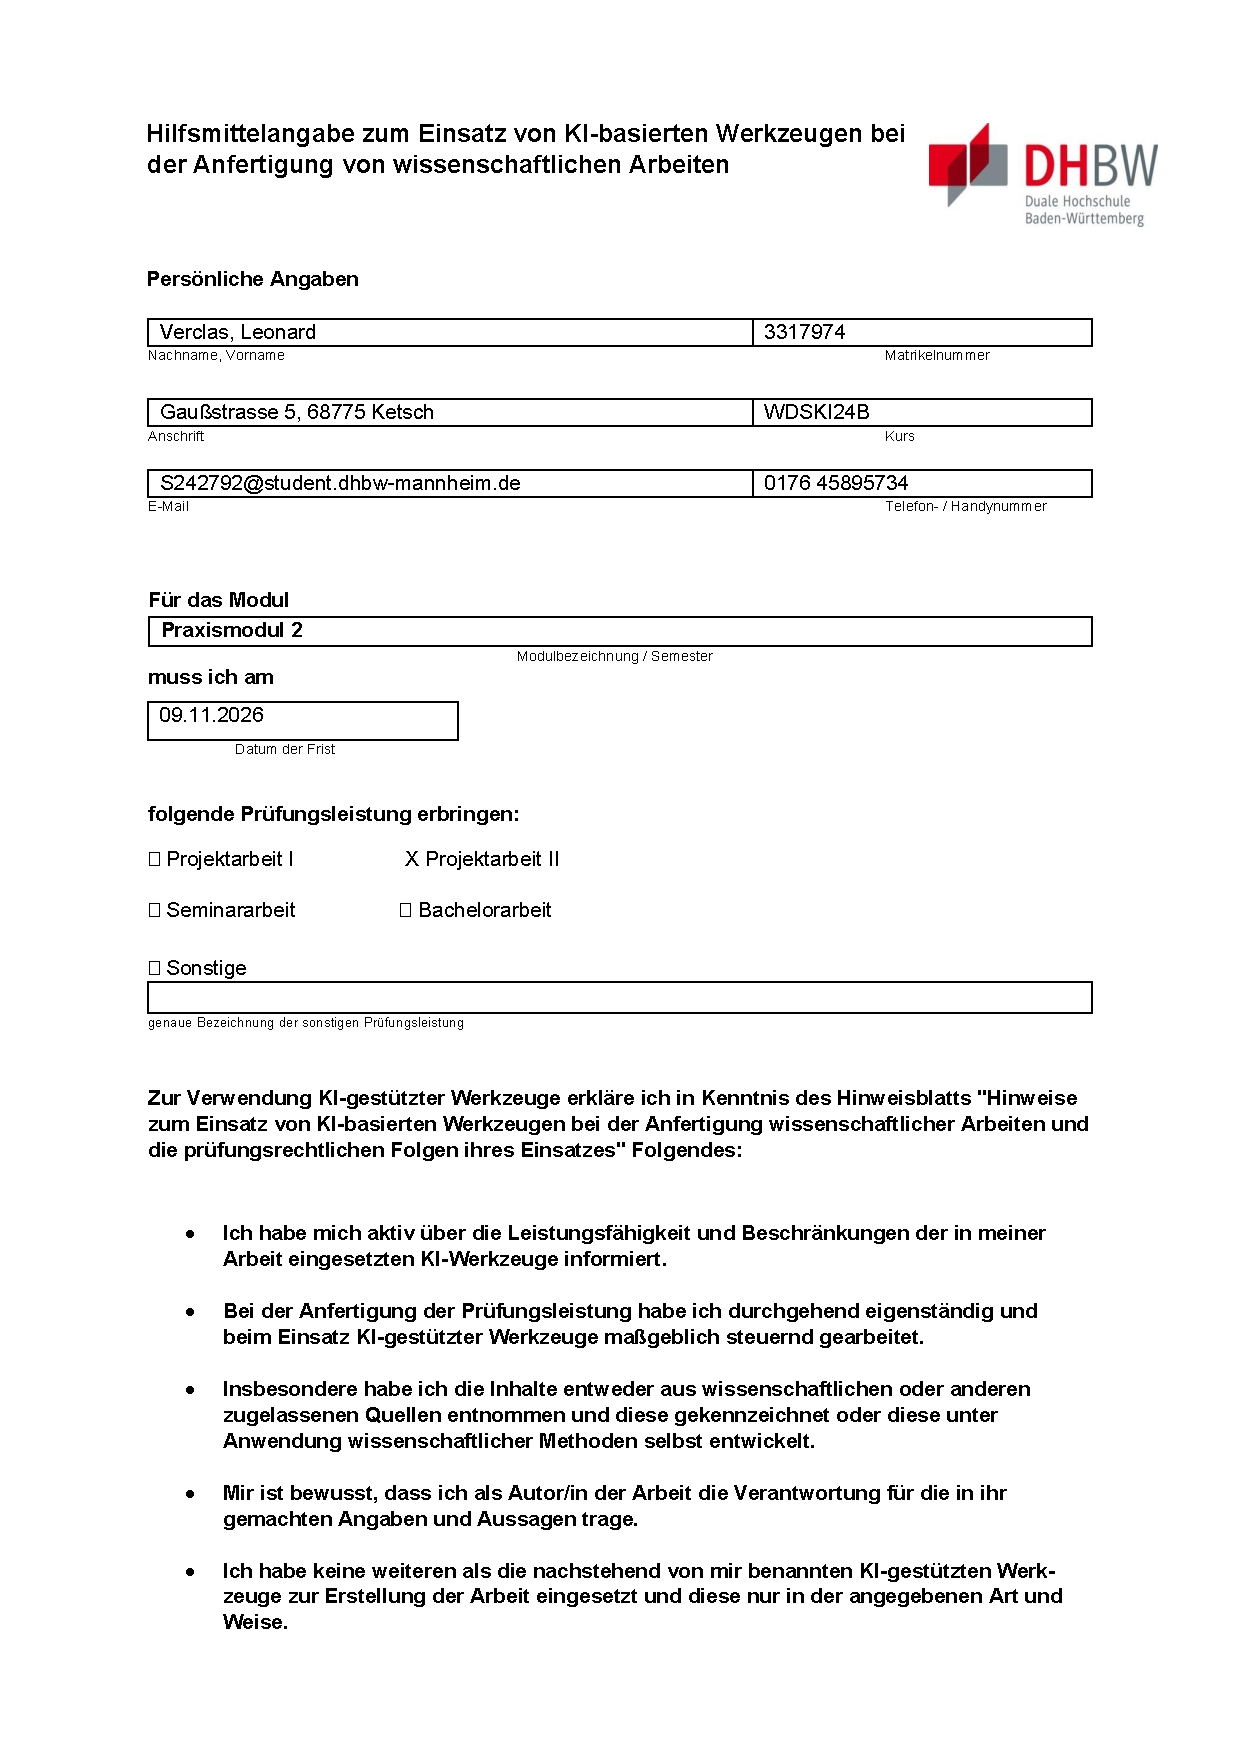
\includepdf[pages=-]{2026_08_03_Formular_Hilfsmittel_KI.pdf}
\end{document}